\documentclass[titlepage]{article}

\usepackage[margin=1in]{geometry}
% some more shit for the title
\usepackage[T1]{fontenc}
\usepackage{babel}

% Tables and stopping them from displaying in a different section
\usepackage{booktabs}
\usepackage[section]{placeins}

% for inserting images into the document, setting file path, and allowing rotation of inserted images 
\usepackage{graphicx}
\graphicspath{ {./images/} }
\usepackage{rotating}
\usepackage[table]{xcolor}
% mostly just for putting text in math equations
\usepackage{amsmath}
% for aligning the text to the left
\usepackage[document]{ragged2e}

% for inserting hyperlinks in the document, use \url{url} or \href{url}{text}
\usepackage{hyperref}
\usepackage{calligra}
\usepackage[T1]{fontenc}
\usepackage{siunitx}
\usepackage{caption}
\usepackage{multirow}
\usepackage[export]{adjustbox}
\usepackage{tikz}
\usepackage{pgfplots}
\pgfplotsset{soldot/.style={color=black,only marks,mark=*},
	             holdot/.style={color=black,fill=white,only marks,mark=*},
		                  compat=1.12}
\usepackage{paracol}

\begin{document}
\title{\textbf{Lab 6: RC Circuits}}
\author{
    Zachary Pouska\\
    \texttt{001103193}\\
    \and
    Natalie Tran \\ 
    \texttt{000698629}\\ \\
} 

\date{PHYS 236 | Fall 2022\\
Date performed: 11/02/2022}


	\maketitle



	\section{Purpose}
    Gaining familiarity with the behavior of capacitors while in both series and parallel with resistors. Understanding of the derived equation to describe the charging and discharging of capacitors. Experimental measurement of the time constant $\tau=RC$.


	\section{Theory}	
    In a DC resistor-capacitor circuit like the figure below, when the switch is connected to position a, the capacitor begins to charge 

    \begin{figure}[hbt!]
        \centering
        \caption{RC series circuit in a neutral position}
        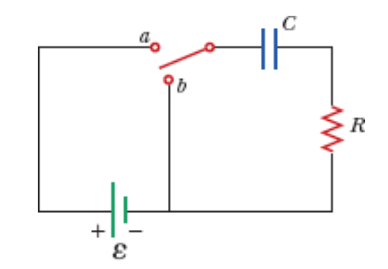
\includegraphics[scale=0.3]{images/theory/circuit.png}
    \end{figure}

    \section{Materials} 
    \begin{enumerate} 
        \item 1 M$\Omega$ resistor
        \item 100$\mu$F polarized capacitor
        \item DC power supply (set at 4V)
        \item Breadboard
        \item Digital multimeter
        \item Dyllan's phone
        \item Numerous alligator clips
        \item Numerous wires 
        \item A single wire that acts as a switch (it's very special)
    \end{enumerate} 


	\section{Experiment Analysis}
    Throughout the experiment, we rely on the following relation between the voltage of the capacitor, the resistance of our resistor, the time constant $\tau$, and time. 
    $$ V_c = \varepsilon (1-e^\frac{-t}{\tau})$$



    \subsection{Linearization of the charging process}
    We start off with our previous equation for the voltage across our capacitor, and begin to manipulate the equation to acquire a more simplified version.


    $$V_c = \varepsilon \left( 1- e^{-\frac{t}{\tau}} \right)  | \div \varepsilon  $$
    $$ \frac{V_c}{\varepsilon}= 1-e^\frac{-t}{\tau}  $$

    



\section{Procedure}
    \subsection{Part 1 - Calculation of the value of the time constant} 
    In this foundational section of the experiment, we measure the functional values of the resistor and the capacitor using the digital multimeter. We then calculated the time constant of our RC circuit using the formula $$\tau = RC$$ and both the theoretical and measure values.
    We finally calculate the percentage error between our theoretical and measure values of the time constant, using the following equation for percentage error. $$\% error = \frac{|\tau_\text{measured} - \tau_\text{nominal}|}{\tau_{nominal}} \times 100$$



    \subsection{Part 2 - Charging the capacitor} 
    After assembling the RC series circuit as displayed in the diagram below and connecting the leads of our multimeter to the leads of the capacitor to get our readouts, we begin the experiment by flipping the switch to the \emph{a} position. When the switch was closed at t=0 seconds, we began recording the voltages across the capacitor at near 5-second intervals. 

    \begin{figure}[hbt!]
        \centering
        \caption{RC series circuit in charging position}
        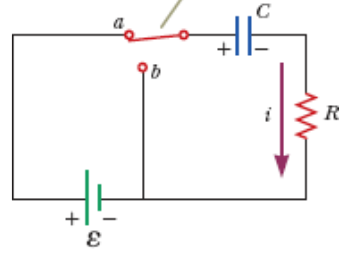
\includegraphics[scale=0.3]{images/procedure/charging.png}
    \end{figure}



    \subsection{Part 3 - discharging the capacitor}
    After performing the previous step of the experiment, we may flip our circuit's switch to the \emph{b} position to begin discharging the capacitor. When the switch is closed at t=0 seconds, we began recording the voltage across the capacitor at roughly 5 second intervals. 




	\section{Data and Graphs}
	\subsection{Part 1}
	\subsection{Part 2} 
	\subsection{Part 3}
	\section{Results}
	\section{Questions}


	\subsection{Part 1}

	\subsection{Part 2}

    \subsection{Part 3}
	
    \subsection{Part 4}
    \begin{enumerate}
        \item Do you obtain the same values for the voltage across the resistor and capacitor? Explain.\\ 
            \textbf{Yes! They are in parallel, so the potential difference across each should be the same. If the potential difference wasn’t equal, that wouldn’t make sense, as measuring the potential difference across each one is essentially connecting the multimeter to the same point in the circuit, assuming 0 resistance in the wires.}
        \item Is the current across the resistor zero? Explain.\\ 
            \textbf{No. In the case of the resistor and capacitor being in series, as the capacitor fills up, it blocks the current flow through the resistor. In this configuration, as the capacitor charges more current is simply diverted through the resistor instead of through the capacitor.}



    \end{enumerate}

	\section{Conclusion}

\end{document}
